\section{Experimental Evaluation}
\label{sec:eval}
% Baba, 5 columns
%     Setup (hw-sw environment, measurement and data collection details)
%     Results
%         Figures, tables: results 
%     Analysis
%     Comparison/contrast with other benchmarks, answers to RQs 
% 

\subsection{Measurement Setup}

For the implementation details, source codes and raw results, see the
benchmark website\footnote{\url{http://incquery.net/publications/benchmarkmetrics}}. In this
section we describe the runtime environment, and highlight some design
decisions.

The benchmark machine contains two quad core Intel Xeon L5420 (2.50GHz) CPU, 32
GBs of RAM and a SAS disk formatted to ext4 for storing the models. In order to
alleviate disturbance of a running measurement and minimize noise in the results,
a bare metal 64 bit Ubuntu 12.04 OS was installed with unnecessary services
(like cron) turned off. OpenJDK JVM version 1.6.0\_24 is used as the Java
environment and Eclipse Juno Modeling 64 bit for Linux for development, and for
the \incquery{} and Java dependencies.

The performance measurements of a tool for a given query-model pair
was independent from the others, i.e. for every tool only its codebase was
loaded, and every scenario measurement (see \figref{fig:asebenchmark}) was run
in a different JVM. Before the execution, OS file cache was cleared, and swap
was disabled to avoid this kind of thrashing. Each test (including all phases)
must be run within 15 minutes, otherwise it was killed.

To obtain faithful execution times, we implemented a benchmarking framework,
which accounted for the time measurements with nanosec precision (that can have
less accuracy!), and the clear separation of phases enforced by the defined
interfaces. These model loading and querying functions were implemented using
functionally equivalent calls of a given tool. See Table~\ref{table:tools} for
the model management format and query language of the benchmarked tools. The
benchmarks were realized as Java applications.

\begin{table}
	\caption{Measured tools}
	\centering
		\begin{tabular}{|l|c|l|r|}
		\hline 
		\textbf{Tool} & \textbf{Model} & \textbf{Query Language} & \textbf{Version}\\ \hline
		Java & EMF & Java & 6.0\\ \hline
		EMF-IncQuery & EMF & IQPL & 0.7.0\\ \hline
		Sesame & RDF & SPARQL & 2.5.0\\ \hline
		 \end{tabular}
	\label{table:tools-met}
\end{table}

Before acquiring memory usage (free heap space) from the JVM, GC calls were
triggered five times to sweep unfreed objects from the RAM. For a JVM, 25 GB
heap limit was specified, but to compensate 64 bit pointers, OOPS (ordinary
object pointers) compression was also turned on: (\code{-XX:MaxPermSize=256m
-XX:+UseCompressedOops -Xmx25g}).

In  the benchmark all cases were run ten times, and the results were dumped into
files, then processed by a spreadsheet software. Finally they are analyzed and
visualized using the R statistical framework.

\subsection{Method of Analysis}
Our long-term goal is providing a catalog of reliable benchmark data that,
based on metrics of the model and the queries, will allow the engineer to
extrapolate the expected performance characteristics of various query
technologies, which in turn will support making an informed decision on the
solution to apply. In scope of this paper, we attempt to provide a necessary
prerequisite with a narrower focus of investigation: finding out which model and
query metrics are useful for predicting the performance 
of the various tools, over a wide range of different queries and model
structures.

A given metric can only be a useful predictor of a certain performance indicator
of a certain tool if they are strongly correlated. Therefore our analysis
investigated correlations of metrics and performance indicators. Neither
previous experience nor current measurement data supported a linear relationship
between these variables; therefore we opted to abandon the commonly used Pearson
correlation coefficient that is associated with linear regression. We rely
instead on Kendall's $\tau$ %and Spearman's $\rho$
 rank correlation coefficient, ranging from $-1$ to $+1$; without assuming a
 linear model, $\tau$ characterises the degree to which it can be said that
 larger values of the metric correspond to larger values of the performance
 indicator.

Correlation coefficients may lead to incorrect conclusions if the sample of
models and queries is too small. Therefore, whenever measuring an absolute value
of $\tau$, we additionally conducted the associated statistical test
($\tau$-test) to decide whether the detected correlation between the variables
is statistically significant ($p<0.001$). Note that any such statistical result
is conditional to the uniform sampling of the selected queries and models.


A limitation of the approach is that two strongly correlated variables (e.g.
\code{countEdges} and \code{countTriples}) may show up as equally good
predictors, but in reality they can not be used as two independent signals for
predicting performance (as most triples in our models are edges). The simple
correlation-based analysis presented here is intended as preliminary feature
selection; we intend to follow up with redundancy-reducing feature selection
techniques such as mRMR~\cite{mRMR-1453511} that can take into account which
metrics convey independent information. Afterwards, predicting the best choice
of technology based on the metric values is a problem of multivariate regression
/ classification, for which we plan to employ advanced machine learning
techniques (e.g. ID3~\cite{ID3-quinlan-1986} decision trees or
MARS~\cite{MARS-MR1091842} regression model) in future work.

\begin{figure*}[tp]
\begin{center}

    \begin{tabular}{c c c}
	    \begin{subfigure}[t]{0.31\textwidth}\centering
	    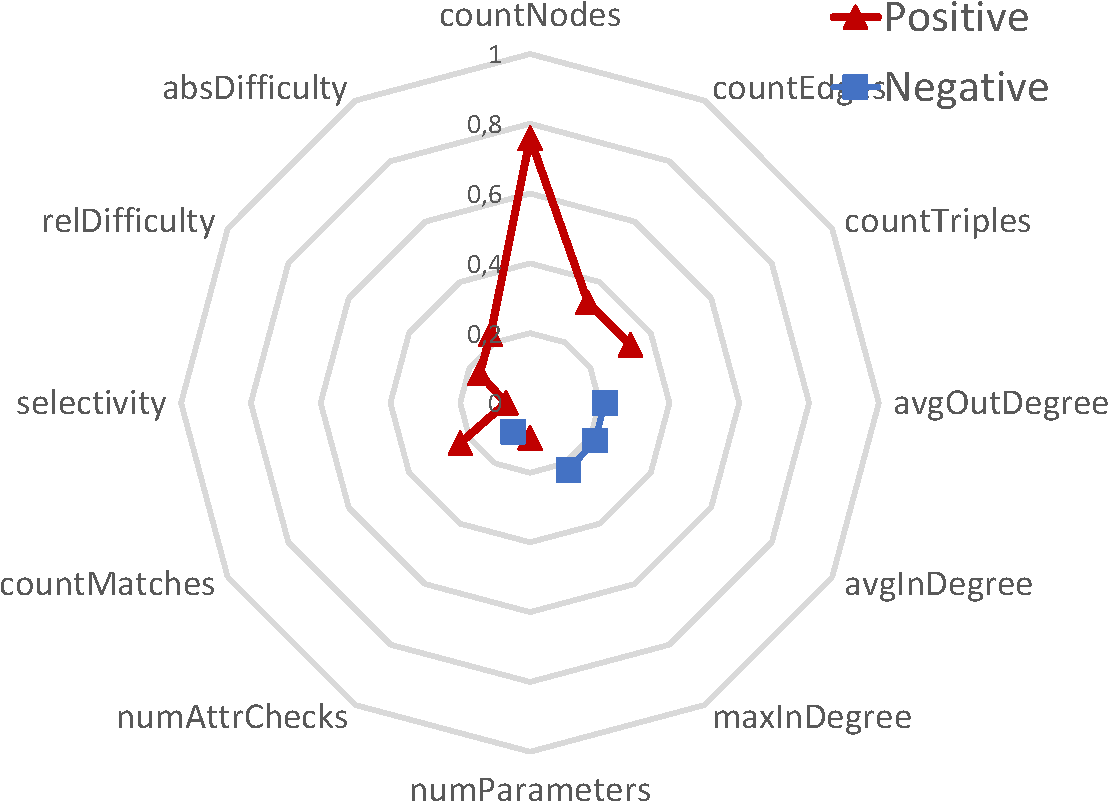
\includegraphics[width=0.95\textwidth]{figures/spider-java-memory.pdf}
	    \caption{Java Memory}\end{subfigure} &
	    \begin{subfigure}[t]{0.31\textwidth}\centering
	    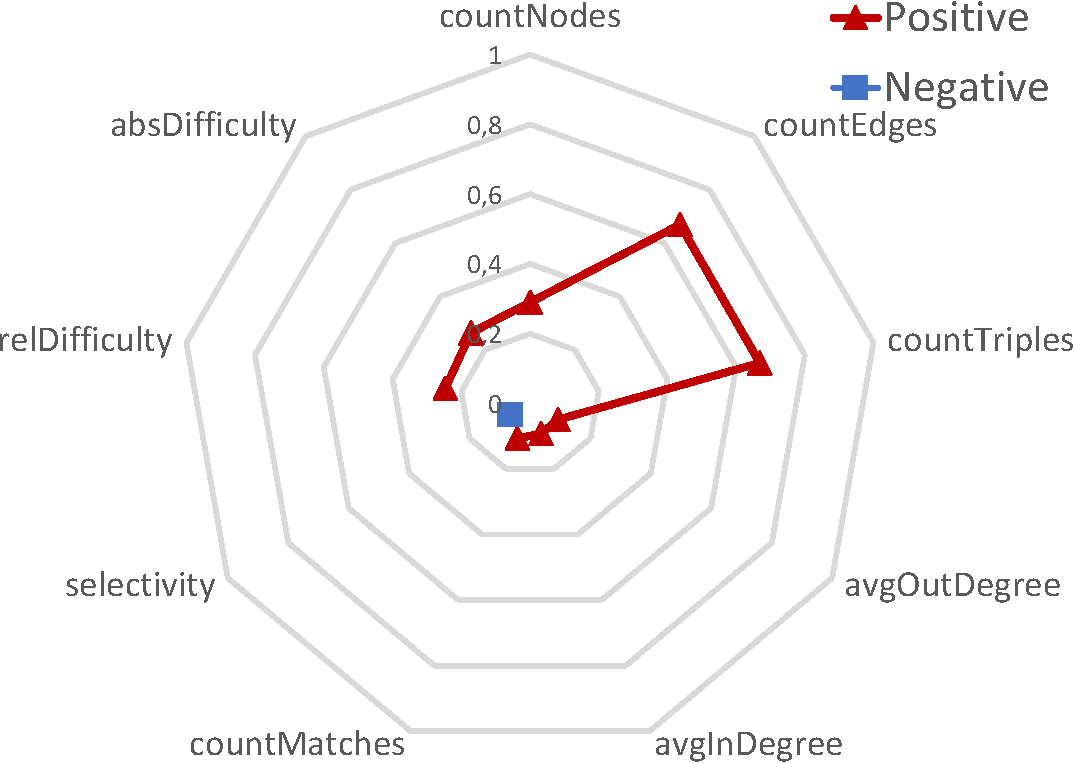
\includegraphics[width=0.95\textwidth]{figures/spider-java-read.pdf}
	    \caption{Java Read time}\end{subfigure} &
	    \begin{subfigure}[t]{0.31\textwidth}\centering
	    \includegraphics[width=0.95\textwidth]{figures/spider-java-check.pdf}
	    \caption{Java Check time}\end{subfigure} \\
	    \begin{subfigure}[t]{0.31\textwidth}\centering
	    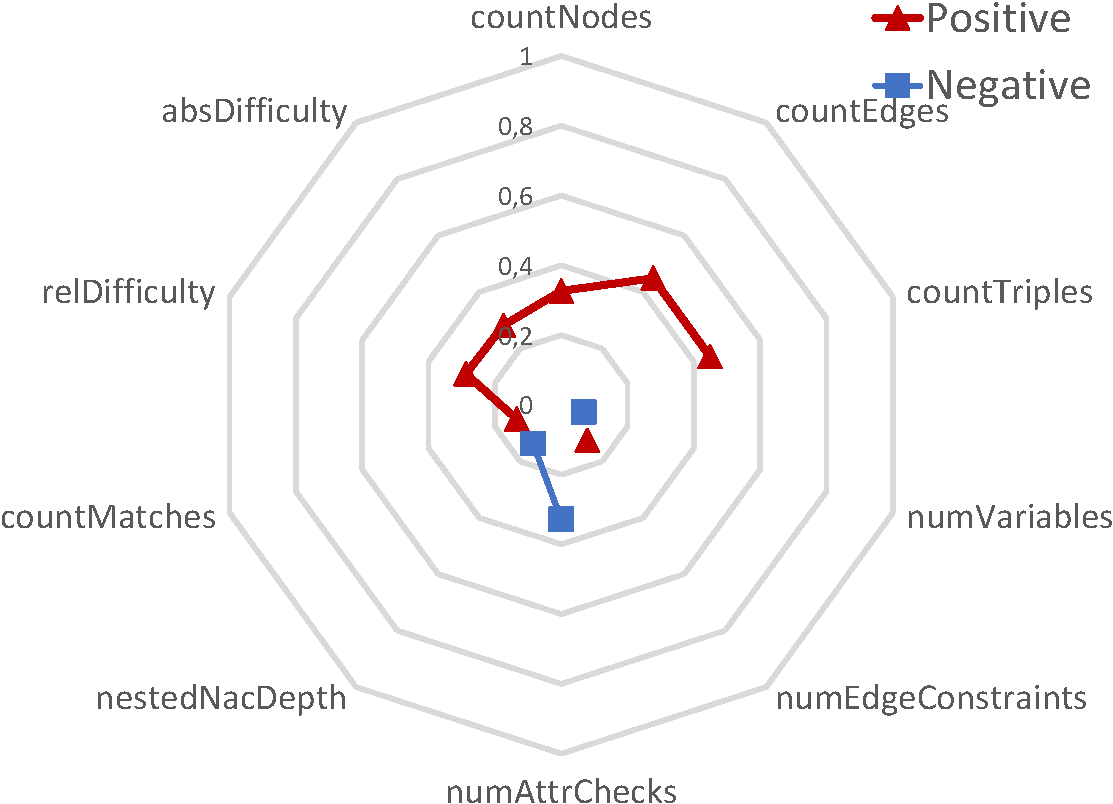
\includegraphics[width=0.95\textwidth]{figures/spider-iq-memory.pdf}
	    \caption{\incquery{} Memory}\end{subfigure} &
	    \begin{subfigure}[t]{0.31\textwidth}\centering
	    \includegraphics[width=0.95\textwidth]{figures/spider-iq-read.pdf}
	    \caption{\incquery{} Read time}\end{subfigure} &
	    \begin{subfigure}[t]{0.31\textwidth}\centering
	    \includegraphics[width=0.95\textwidth]{figures/spider-iq-check.pdf}
	    \caption{\incquery{} Check time}\end{subfigure} \\
	    \begin{subfigure}[t]{0.31\textwidth}\centering
	    \includegraphics[width=0.95\textwidth]{figures/spider-sesame-memory.pdf}
	    \caption{Sesame Memory}\end{subfigure} &
	    \begin{subfigure}[t]{0.31\textwidth}\centering
	    \includegraphics[width=0.95\textwidth]{figures/spider-sesame-read.pdf}
	    \caption{Sesame Read time}\end{subfigure} &
	    \begin{subfigure}[t]{0.31\textwidth}\centering
	    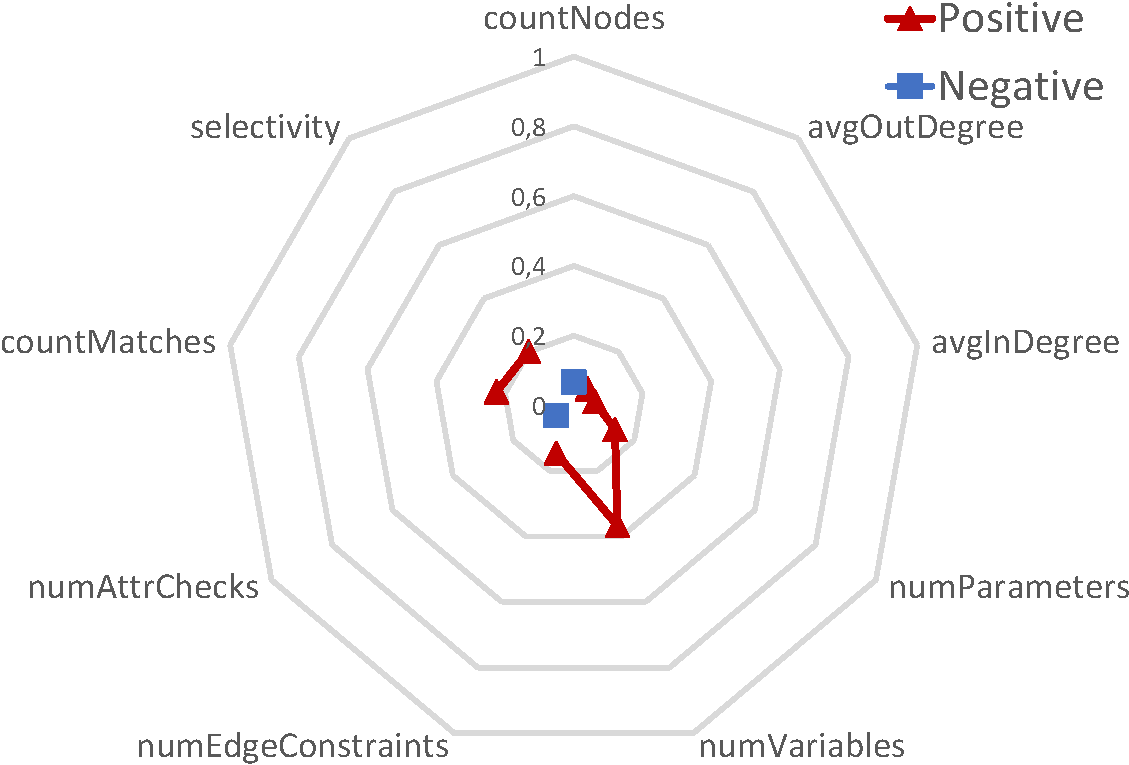
\includegraphics[width=0.95\textwidth]{figures/spider-sesame-check.pdf}
	    \caption{Sesame Check time}\end{subfigure} 
    \end{tabular}
  \caption{$\abs{\tau}$ of correlating ($p<0.001$) metrics for each performance indicator}
  \label{fig:correlation-spider}
\end{center}
\end{figure*}

\subsection{Results}
For each tool performance indicator and each metric, we conducted Kendall's correlation test to see whether the data available is sufficient to form a statistically significant support of correlation between the performance indicator and the metric. For metrics that were found to correlate, the absolute value of Kendall's $\tau$ correlation coefficient is displayed on a spider chart specific to the performance indicator of the tool (see \autoref{fig:correlation-spider}); positive correlation values are displayed as red triangles, while negative ones as blue squares.  

\subsubsection{Evaluation}
Consistently with previously published results, the data shows that model size is a strong predictor of both model loading time and memory consumption, regardless of the technology.
\paragraph{Tool-specific Observations}
However, check times show a more diverse picture. The check times for the Java implementation (being a dominantly search-intensive approach) are additionally correlated with the query-on-model metrics as well, with the strongest correlation shown by the \emph{absDifficulty} metric. 

Interestingly, the best Sesame check time predictor turned out to be the number of pattern variables, and there is no significant correlation with any direct model metrics. 

Check times in \incquery{} are very strongly correlated to the number of matches - which is to be expected of an incremental tool whose check phase consists of just enumerating the cached match set. As the incremental indexes are constructed during the load time, the model-on-query metrics become correlated with \incquery{} read time. It can also be highlighted that \incquery{} seems not to be sensitive towards the ``difficulty'' of the query (in any phase) or the model size (during the check phase) due to the very small correlations with corresponding metrics.
\paragraph{Metrics}
Overall, it can be said that model-only metrics are useful in predicting the performance of model persistence operations. However, query-based and combined metrics (such as our proposed \emph{abs-} and \emph{relDifficulty}) are necessary to provide a more thorough picture.
Note that since only statistically significant correlations are included, a low magnitude correlation does not necessarily mean a measurement error. It is possible that there is a true link between the two variables, but the $\tau$ value is lowered by other metrics that strongly influence the performance indicator. 
% \paragraph{Decision making}
% The Goal Question Metric (GQM) approach~\cite{gqm} can be used to make informed decisions about tool or language selection. A \emph{goal} can be that the processing of models must be efficient. \emph{Questions} would be: batch or incremental scenario is performed by the tools? How large is the model? What is the complexity of the queries? These can be answered using the relevant metrics of Fig. \ref{fig:correlation-spider}. Metrics with high correlation will have the most impact on runtime. In the future we plan to extend this benchmark, and build decision trees or more complex decision support systems that can aid domain engineers to choose the right tool and languages for their task.

% [5/18/13 8:29:53 AM] Varró, Daniel: Toolokról külön-külön kellene írni valamit
% [5/18/13 8:30:26 AM] Varró, Daniel: továbbá a végén arról, hogy a szakirodalomból ismert metrikák mennyire bizonyultak használhatónak vagy használhatatlannak
% [5/18/13 8:31:12 AM] Varró, Daniel: A negatív eredményeket / meglepetéseket is el kellene magyaráznunk, nemcsak a pozitív korrelációt

\subsubsection{Threats to Validity}
Regarding the technological foundations and methodology of our measurements, the
most important threats to validity stem from \emph{time measurement uncertainty}
and distortions due to transient effects such as \emph{garbage collection} in
the JVM and \emph{thrashing} due to heap size exhaustion. Such effects were
mitigated by using the most accurate Java time measurement method
(\code{System.nanoTime}), allocating as much heap as possible, and using a
timeout mechanism to identify and exclude cases affected by thrashing from the
results.
Additionally, it is also possible that there is sampling bias in our choice of
models and metrics; we believe that this is sufficiently mitigated by our
systematic choice of model generation strategies and the design principles of
the queries. To improve the magnitude of correlation we increased the sample
size by running the benchmarks ten times.